\chapter{Versuchsdurchführung}

    \section{Charakterisierung des Cantilevers}

Zur Mikroskopierung einiger Proben wird in diesesm Versuch der dynamische Modus des
Mikroskops verwendet. Dies erfordert Kenntnis über das dynamische Verhalten des 
Cantilevers. Daher soll die Resonanzkurve aufgezeichnet und daraus die Güte der
Messspitze bestimmt werden. \par
\begin{figure}[hb]
    \centering
    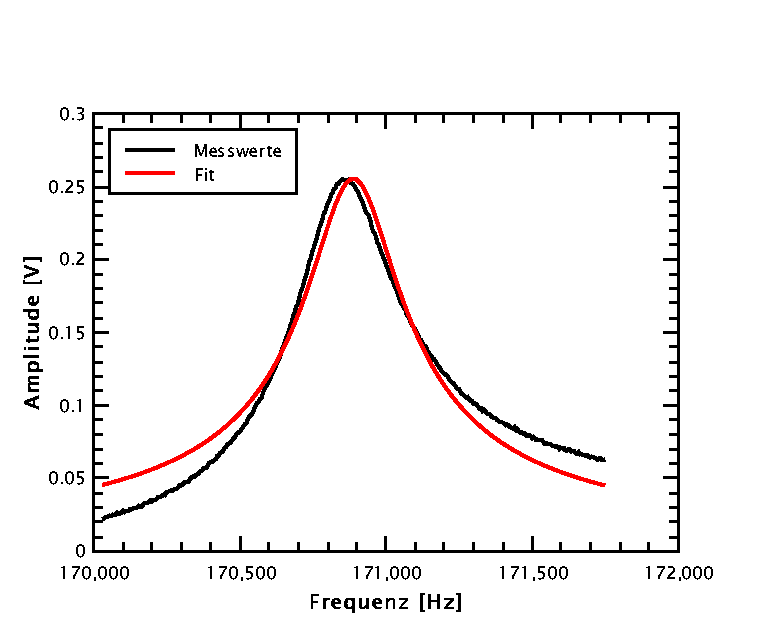
\includegraphics[width=0.6\textwidth]{Mess/freqsweep_2.pdf}
    \caption{Resonanzkurve des Cantilevers gefittet mit Gleichung des getriebenen,
             gedämpften Oszillators}
    \label{freqsweep}
\end{figure}
In Abbildung \ref{freqsweep} ist die aufgenommene Resonanzkurve zu sehen, gefittet
mit der Formel
\[
    A(\omega) = \frac{F_0}{m \sqrt{(\omega_0^2 - \omega^2)^2 + \left( 
    \frac{\omega\omega_0}{Q} \right)^2} }
\]
des getriebenen, gedämpften Oszillators, siehe Kapitel \ref{herleitung} für die 
Herleitung. Aus dem Graphen lassen sich einige Werte
bestimmen, die im weiteren Verlauf des Versuches nützlich sein werden.
\begin{align*}
    Q=551,8 & & \frac{F_0}{m} = \SI{13,5}{MN\per\kg} & & \omega_0 =
    \SI{170,9}{kHz}
\end{align*}
$Q$ bezeichnet hierbei den Gütefaktor des Cantilevers und $\omega_0$ die 
Resonanzfrequenz. 
\vspace{6pt}\\
Anders als theoretisch errechnet, ist die gemessene Kurve nicht ganz symmetrisch.
Dies ist auf die Annäherung des Messkopfes als Massepunkt zurückzuführen.

    \section{Überprüfung der Geräteparameter}

Um Entfernungen auf Proben messen zu können, müssen die an den Piezo angelegten 
Spannungen zuverlässig in $x$, $y$ und $z$ Auslenkungen umgerechnet werden können.
Um diese Kalibrierung zu überprüfen, wird ein Eichgitter mit einer Gitterperiode
von  $\SI{10}{\mu m}$ verwendet.
\begin{figure}
    \centering
    \begin{subfigure}[hb]{0.4\textwidth}
        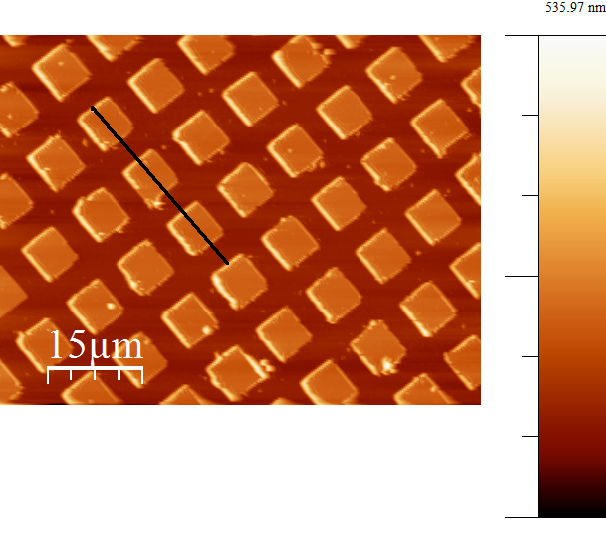
\includegraphics[width=\textwidth]{Mess/gitter_paint.png}
        \caption{Topographie des Eichgitters; Messung des Gitters eingezeichnet}
        \label{gitter}
    \end{subfigure}
    \begin{subfigure}[hb]{0.4\textwidth}
        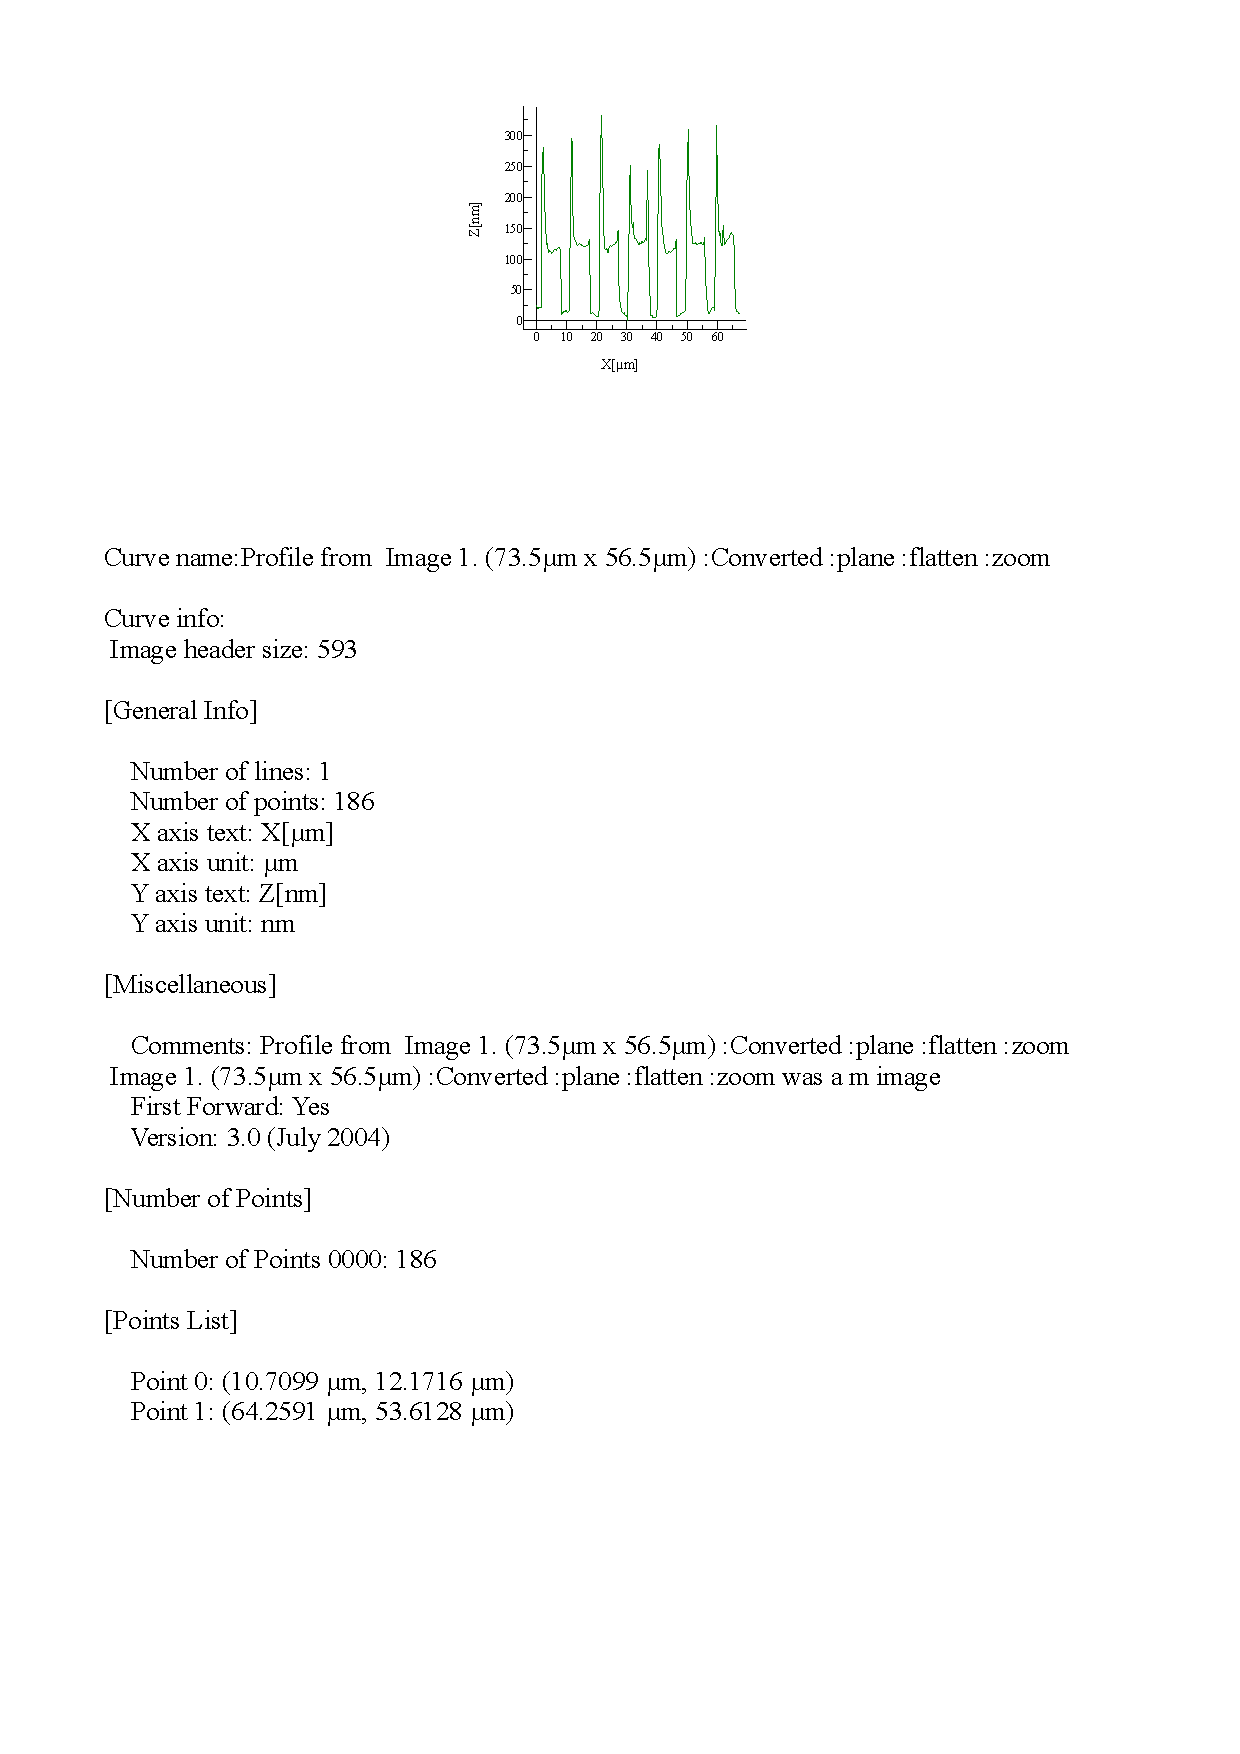
\includegraphics[width=\textwidth]{Mess/profil_gitter.pdf}
        \caption{Horizontales Profil des Gitters}
    \end{subfigure}
    \caption{Spektroskopie des Eichgitters}
\end{figure}
In Abbildung \ref{gitter} ist eine Teilaufnahme des Gitters zu sehen. Der Abstand 
zweier Quadrate beträgt laut Messung $\SI{10,7}{\mu m}$. Dies ist ein gutes 
Ergebnis, weshalb die Default-Werte im weiteren Verlauf des Versuch verwendet 
werden.

    \section{Spektroskopie}

Nun soll die Amplitude der oszillierenden Messspitze bestimmt werden. Hierzu wird
der Scankopf über einer homogenen Oberfläche positioniert und die Änderung der 
Schwingungsamplitude bei Annäherung an die Probe aufgezeichnet.
\begin{figure}[hp]
    \centering
    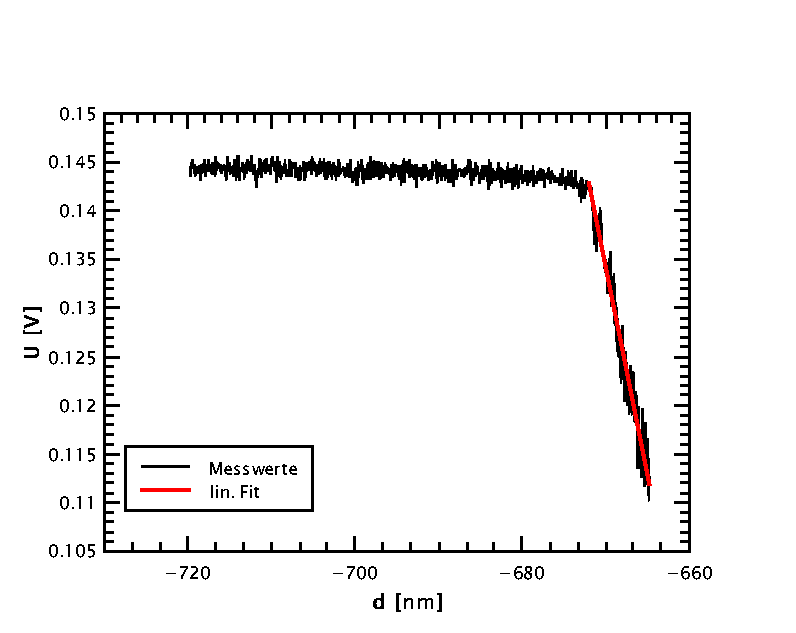
\includegraphics[width=0.6\textwidth]{Mess/spek_forw.pdf}
    \caption{Vorwärts-Spektroskopie}
    \label{spek_forw}
\end{figure}
\begin{figure}[hp]
    \centering
    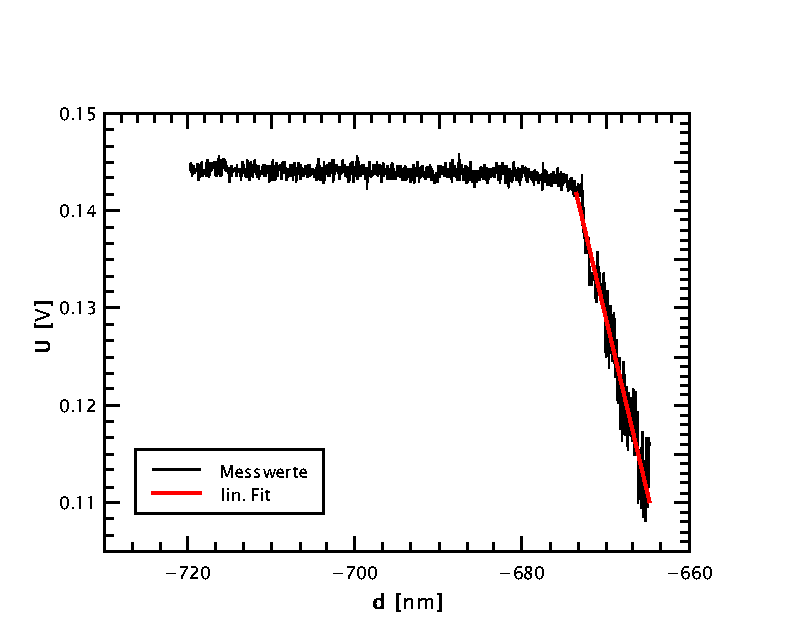
\includegraphics[width=0.6\textwidth]{Mess/spek_backw.pdf}
    \caption{Rückwärts-Spektroskopie}
    \label{spek_backw}
\end{figure}
In den Abbildungen \ref{spek_forw} und \ref{spek_backw} sind diese Messungen, erst
bei Annäherung an die Probe, dann bei Entfernung von der Probe, zu sehen. Die 
Amplitude ist bei großen Entfernungen nahezu konstant. Bei Kontakt zwischen Spitze
und Probe befindet sich der untere Umkehrpunkt der Oszillation an der 
Probenoberfläche.
Somit sinkt die Amplitude um die Änderung der z-Position. Dieser lineare 
Zusammenhang zwischen Höhe des Cantilevers und der Amplitude soll nun zur 
Bestimmung der Amplitude benutzt werden.
\vspace{6pt}\\
Aus den linearen Fits kann die Proportionalitätskonstante für beide Messungen
bestimmt werden.
\begin{align*}
    K_{\text{for}} = \SI{4,27e6}{A s \per N} & & K_{\text{rück}} = 
    \SI{5,61e6}{A s \per N}
\end{align*}
Mithilfe der Formel $\displaystyle A = \frac{U}{K}$ und der Spannung vor Annäherung
an die Probe von $U \approx \SI{140}{mV}$ kann die Amplitude zu
\begin{align*}
    A = \frac{U}{K} \approx \frac{\SI{140}{mV}}{\SI{4,936e6}{A s \per N}} = \SI{29,2}{nm}
\end{align*}
bestimmt werden.

    \section{Spur-Abstand einer CD}

Zuletzt wird mithilfe des Mikroskops die Kapazität einer CD bestimmt. Hierzu
soll die Spurbreite und der Bitabstand bestimmt werden, um die Fläche eines 
Datenpunktes zu errechnen. Kennt man die Spurlänge über die komplette CD, kann so auf die Kapazität 
geschlossen werden. \par
\begin{figure}
    \centering
    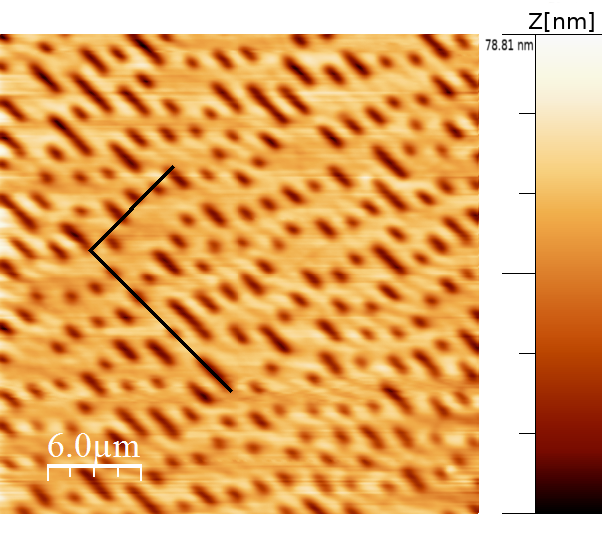
\includegraphics[width=0.6\textwidth]{Mess/cd_paint.png}
    \caption{Topographie der Datenseite einer CD; Messung eingezeichnet
             Pitlänge wird durch die lange Linie, Spurabstand durch die
             im 90$^\circ$ dazu stehende kürzere Linie gemessen}
    \label{cd}
\end{figure}
Aus Abbildung \ref{cd} kann der Spurabstand zu $\SI{1,29}{\mu m}$ und die
Pitlänge zu $\SI{1,42}{\mu m}$ bestimmt werden. 
Die tatsächliche Pitlänge beläuft sich auf die Hälfte der gemessenen, also
$\SI{0,71}{\mu m}$ (Übergangsbereich). Dies entspricht nun der Länge eines
Bits auf der CD. Weiter gilt es zu beachten, dass auf einer CD 17 Bits zur
Speicherung eines Bytes verwendet werden, statt den herkömmlichen 8 auf 
Festplatten. Innen- und Außenradius sollen als $r_i = \SI{2,2}{cm}$ und 
$r_a = \SI{5,9}{cm}$ angenommen werden. 
\vspace{6pt}
Zur Berechnung der Kapazität wird eine spiralförmige Spur von Bits auf der CD
angenommen. Verwendet werden die gemessenen Größen Spurabstand $s$ und 
Bitlänge $l$.
\[
    \vec{r}_n = (r_i+s \, n) 
        \begin{pmatrix}
            \sin(2\pi n)\\
            \cos(2\pi n)
        \end{pmatrix}
\]
Für die Gesamtlänge ergibt sich somit
\[
    L = \frac{2d}{d} \int_0^N dn | \dot{\vec{r}} | = \int_0^N dn \, s
        \sqrt{1 + 4 \pi^2 \left( \frac{r_i}{s} + n \right)^2} 
\]
N steht hierbei für die Gesamtanzahl der Spuren
\[
    N = \frac{r_a - r_i}{s} = 28682
\]
Hiermit errechnet sich die gesamte Länge der Spirale zu $\SI{7299}{m}$.
Für die Kapazität ergibt sich somit
\[
    \text{Kapazität} = \frac{L}{17 \cdot l \cdot 1024^2} = \SI{577}{MB}
\]
Die Abweichung von $11 \%$ kommt wohl durch das unscharfe Messbild, aus
dem die tatsächliche Pitlänge und Spurabstand nur schwer bestimmt werden konnten,
sowie einer tatsächlich niedrigeren Kapazität der CD zustande.
